\documentclass[14pt, titlepage,fleqn]{extarticle}
\usepackage[T1,T2A]{fontenc}
\usepackage[utf8]{inputenc}

\usepackage{amsmath}
\usepackage[russian]{babel}

\usepackage{titlepage}
\usepackage[final]{pdfpages}
\usepackage{listings}
\usepackage{color}
\usepackage{graphicx}
\usepackage{float} 

\usepackage{caption}


\newcommand{\InsertGraf}[2]{
	\begin{figure}[H]
		\center{\includegraphics[width = 1\textwidth]{#1}}
		\caption{#2}
	\end{figure}
}

\definecolor{dkgreen}{rgb}{0,0.6,0}
\definecolor{gray}{rgb}{0.5,0.5,0.5}
\definecolor{mauve}{rgb}{0.58,0,0.82}


\lstset{frame=tb,
	language=Python,
	aboveskip=3mm,
	belowskip=3mm,
	showstringspaces=false,
	columns=flexible,
	basicstyle={\small\ttfamily},
	numbers=none,
	numberstyle=\tiny\color{gray},
	keywordstyle=\color{blue},
	commentstyle=\color{dkgreen},
	stringstyle=\color{mauve},
	breaklines=true,
	breakatwhitespace=true,
	tabsize=3
}

\begin{document}
	\selectlanguage{russian}
	

	\fefutitlepage{Б9119-02.03.01сцт}{Панченко Н.К.}{02}{июня}{22}
	
	
	\newpage
	
	\tableofcontents   
	\clearpage
	\section*{Введение}
	\addcontentsline{toc}{section}{Введение}
	Отчёт по лабораторной работе на тему <<Метод Ричардсона>>.	
	\newpage









	\section*{Метод Ричардсона}
	\addcontentsline{toc}{section}{Метод Ричардсона}
	Изучить и реализовать метод Ричардсона для решения СЛАУ, а также описать работу алгоритма и
	привести результаты.

	\section*{Алгоритм}
	Найти минимальное и максимальное собственные значения матрицы:
	\[a = min(\lambda_i(A)), b = max(\lambda_i(A))\]	
	\[\tau^{0}_i = \dfrac{2}{(a + b) + (b-a)\cos\left(\dfrac{(2i-1)\pi}{2n}\right)},~~~i=1,2,...,k; \]
	\[x^{k+1} = x^k = \tau_{k+1}Ax^k + \tau_{k+1}f\]
	\section*{Тесты}
	Возьмем матрицу:
	\[A = \begin{pmatrix}
		16& 2& 0& -2\\
        4& 20& 1& 0\\
        2& 0& 10& 0\\
        -4& 0& 4& 32
	\end{pmatrix}\]
	Возьмем вектор:
	\[b =\begin{pmatrix}
		13\\
		24\\
		7\\
		0
	\end{pmatrix} \]
	\newpage
	Результаты при $n=10$ и $\epsilon = 10^{-2}$:
	\begin{figure}[H]
		\center{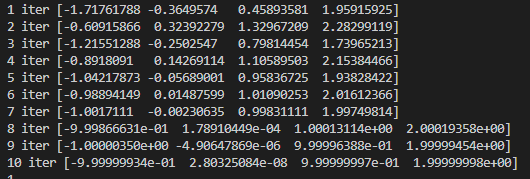
\includegraphics[width = 1\textwidth]{Screenshot_1.png}}
	\end{figure}
\end{document}